\chapter{Results}
\label{ch:results}

- High level overview on how the plots were made (refer to flow chart)
- Explain rationale as it allows easy visual inspection
- Describe how plots were designed: what we are looking for in each column
- Delineation against land cover on left and middle plots potentially indicates that land cover is responsible for the observed differences
- Delineation against plots on right leaves open the question of what is causing the change, but suggests the change is being modulated by the presence of land cover
- Trend on right plot which correlate with changes in vegetation suggest that land cover may be responsible for the observed differences.

\section{General}

\subsection{Orography}

For reference, the orography for each focus region is displayed in Figure~\ref{fig:orog}.

\begin{figure}[!ht]
	\centering
	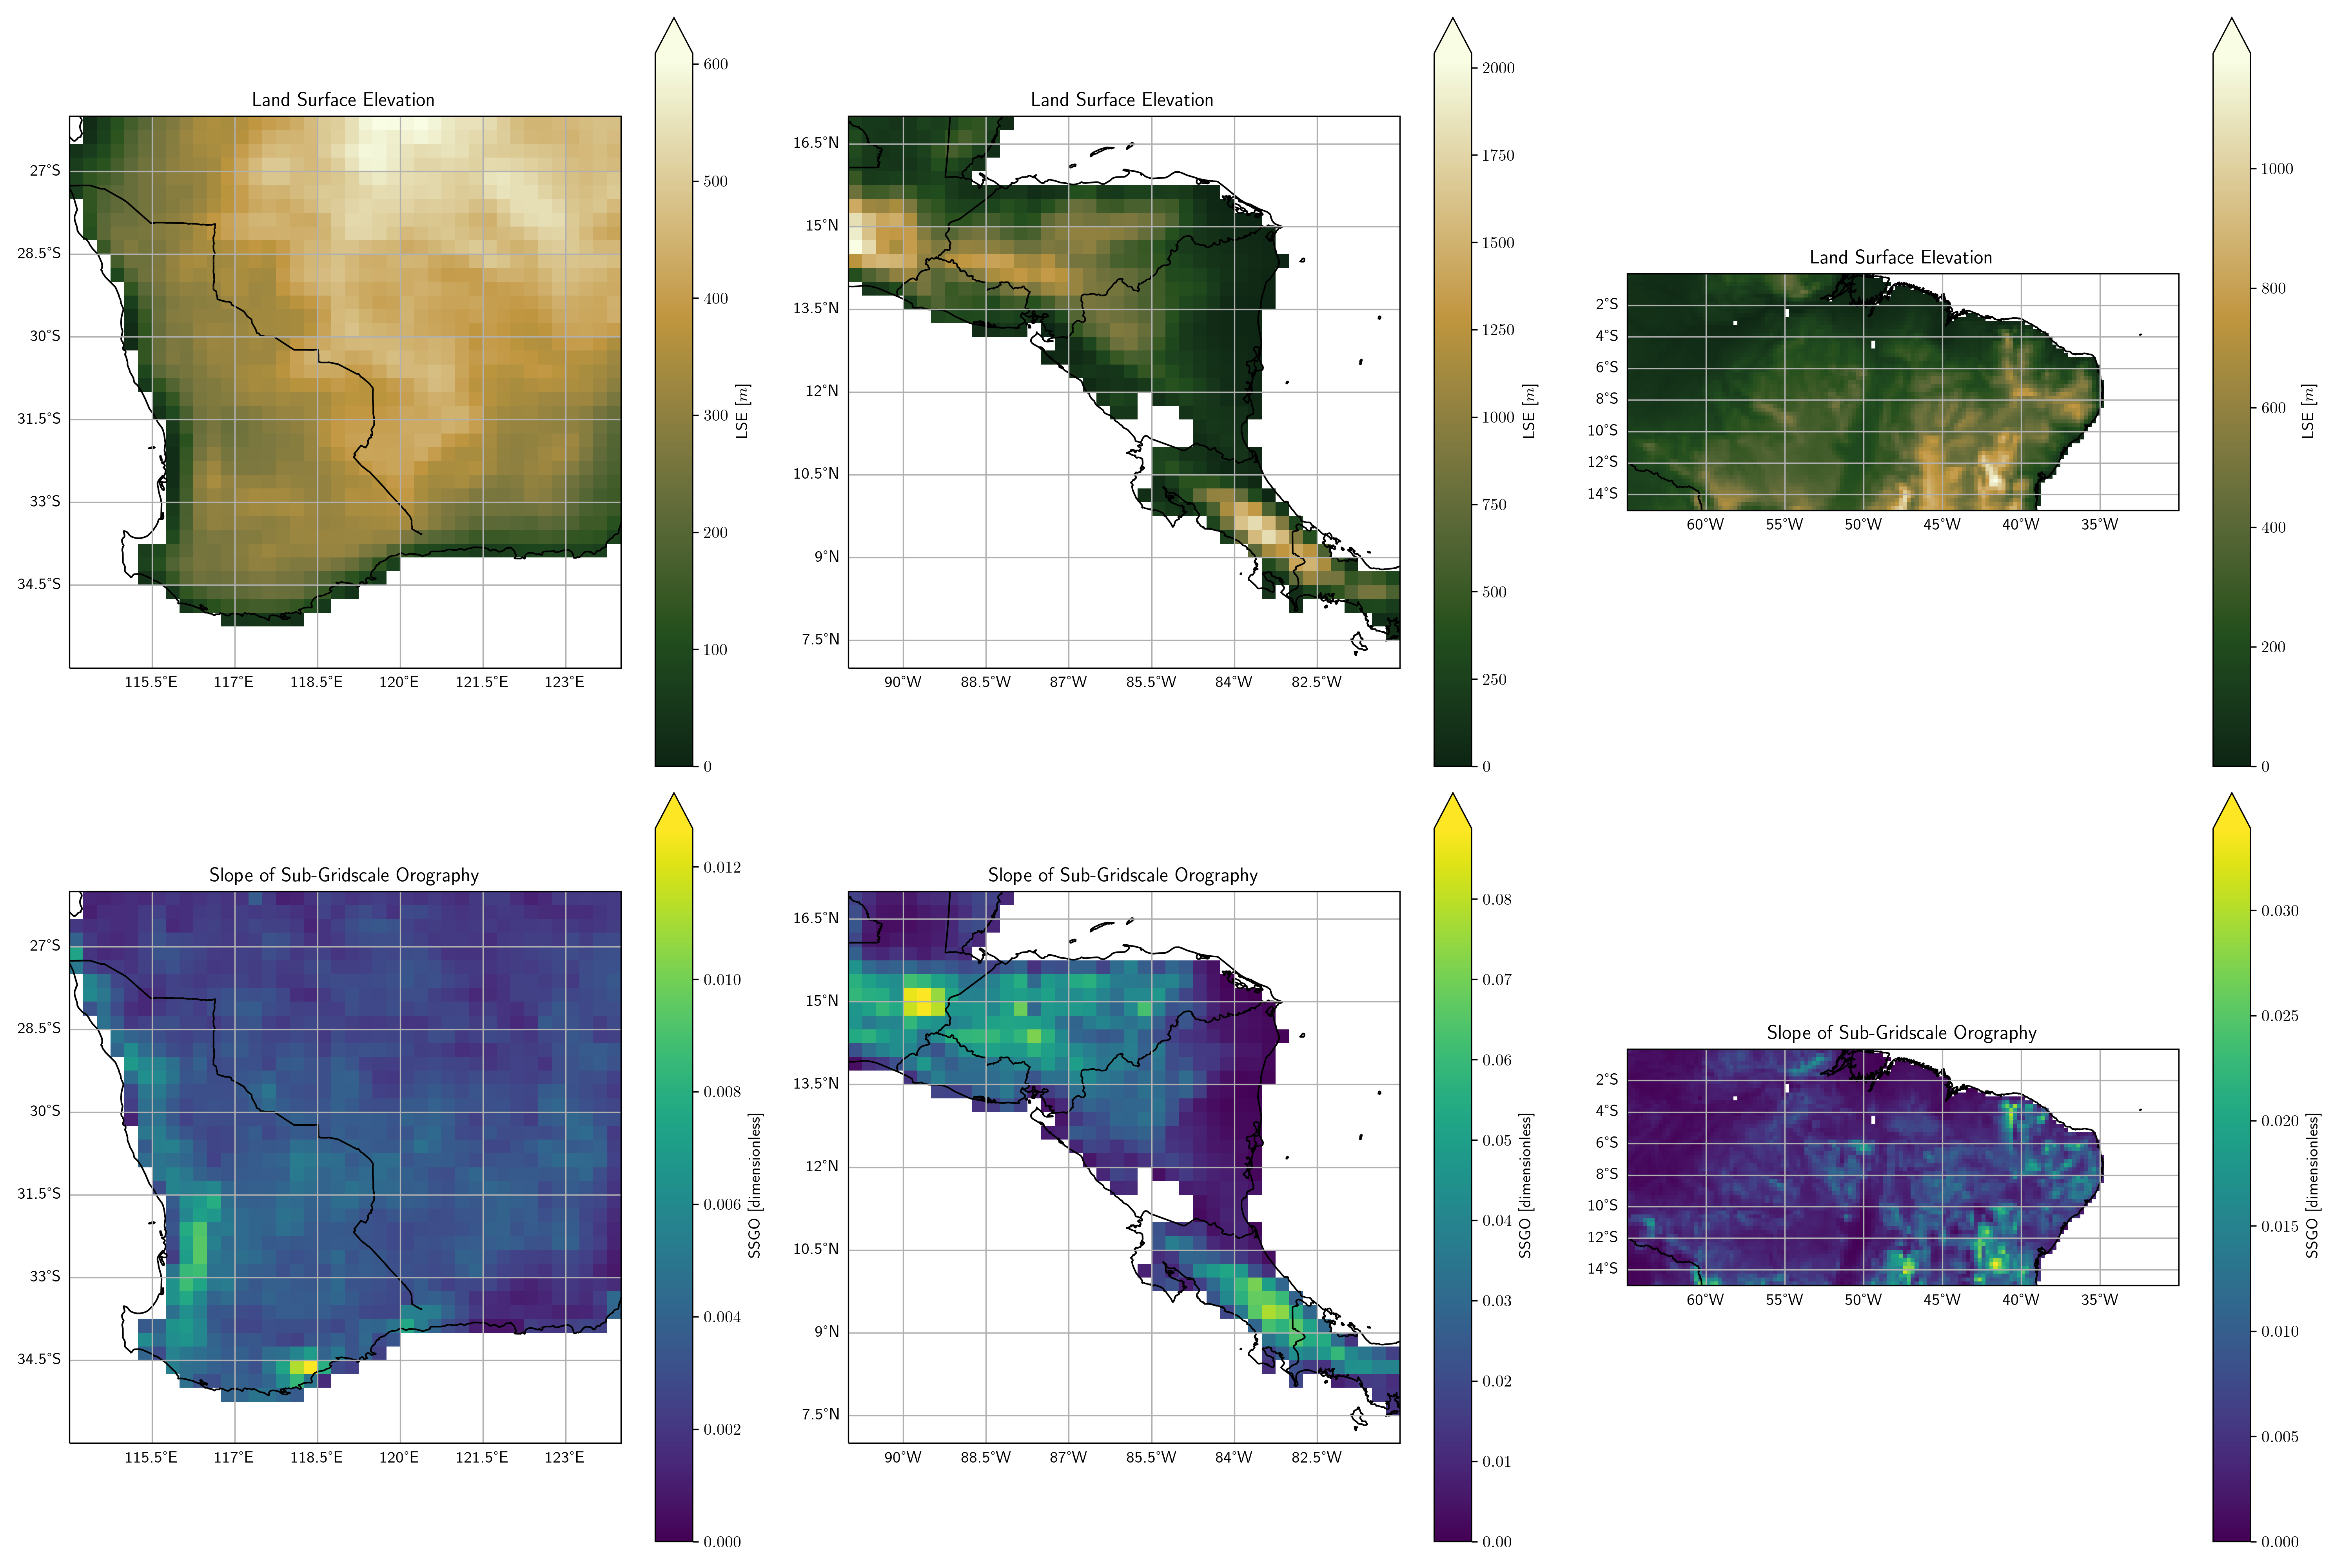
\includegraphics[width=0.9\textwidth]{orog.png}
	\caption[Orography for each focus region]{Top row: \acf{LSE} for each region. Bottom row: \acf{SSGO} for each region. From left to right: \acl{WA}, \acl{CA}, \acl{NB}.}
	\label{fig:orog}
\end{figure}

\section{Western Australia}
\label{sec:results_wa}

\subsection{Selected results from similar comparison}

\subsubsection{Study periods}

For \ac{WA}, the selected periods for the similar comparison was from Jun-1997 to May-2002 and from Sep-2010 to Aug-2015. 

Between these periods was extensive vegetation loss concentrated along the coastal forests, resulting from a mix of drought events and human activities such as mining and forestry (beyond vegetation clearing, these activities are also implicated in causing a drop in the region's water table). The main climate drivers for this region are the \ac{IOD} and \ac{AAO} (also known as \ac{SAM}) \citep{wa_drivers}. The corresponding indices are the \ac{DMI} and \ac{AAOI} respectively, and these = have similar averages over these periods. In fact, the 5-year averages over all the indices apart from the \ac{EPOI} (which is distant and not expected to have significant effects) have very similar values (not shown), although they appear to span across different phases for the longer-term oscillations.

The period from Jun-1997 to May-2002 contains one Negative \ac{IOD} event and one Positive \ac{IOD} event, both of which display relatively high magnitudes for monthly values. Although the period from Sep-2010 to Aug-2015 contain two Negative \ac{IOD} events and two Positive \ac{IOD} events, each of these display relatively low magnitude in monthly values and so should still be comparable against the first period.

\subsection{Diurnal comparison for January}

\subsubsection{VIEC delineation along fence.}

\ac{VIEC} mean values computed over January displayed a marked distinction across the \acf{SBFWA}, with more strongly negative values on the native side of the fence during both the day and night (see Figure~\ref{fig:wa_jan_comb_1}).\footnote{The following results are also observed to varying degrees for the months of February, October, November and December, but we present January because this month displays these trends most distinctly.} During daytime, this also marks the distinction between positive \ac{VIEC} values on the agricultural side and negative values on the native side. Negative $\ac{VIEC}$ values indicate a greater prevalence for upwards air movement (kinetic energy converted into gravitational potential energy), while positive values indicate the opposite.\footnote{There are better variables than \ac{VIEC} in the ERA5 dataset to analyse upwards/downwards air movement since \ac{VIEC} lumps internal and gravitational potential energy together, but these other variables were not included in the original analysis and time constraints in this project did not allow for modification of the methodology.}

\begin{figure}[!ht]
	\centering
	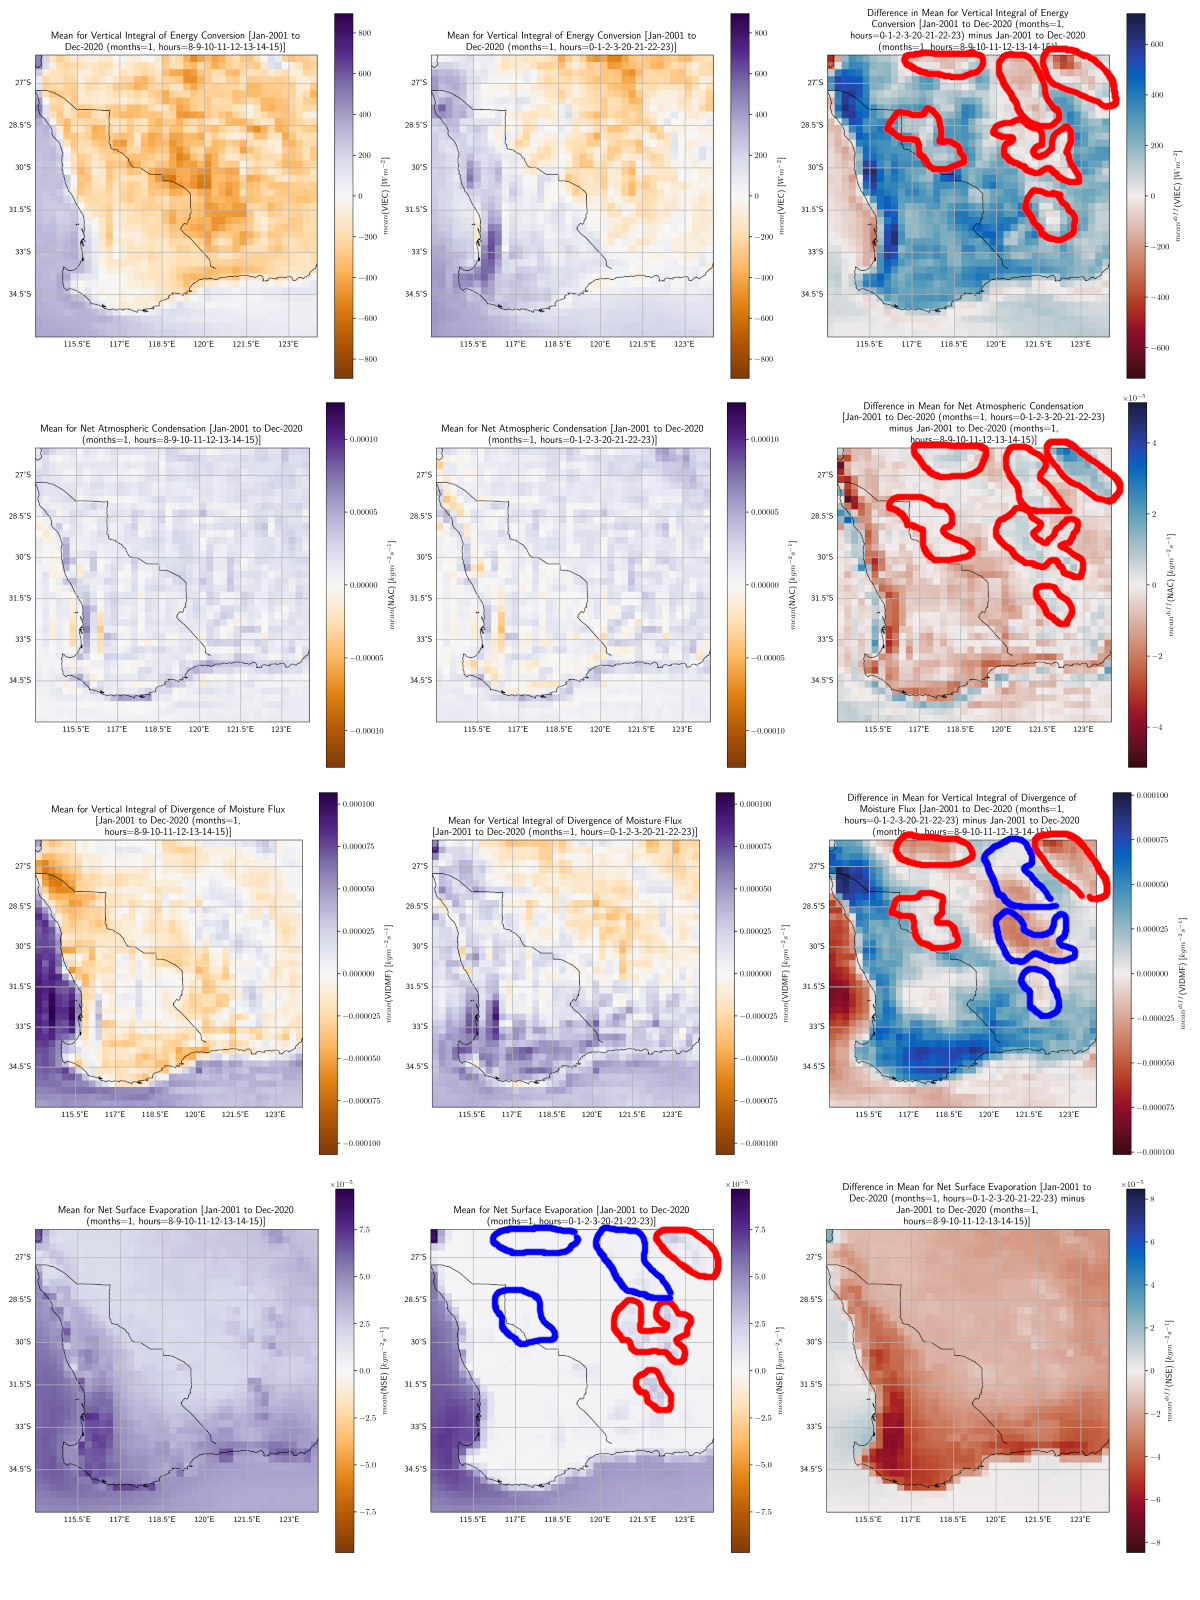
\includegraphics[width=0.9\textwidth]{wa_jan_comb_1.png}
	\caption[WA January means for selected variables 1]{January mean daytime and nighttime values for \acs{VIEC}, \acs{NAC}, \acs{VIDMF} and \acs{NSE}. Red markings indicate selected areas which are distinct from background trends. Blue markings indicate areas where such a distinction did not exist, but did exist for \acs{VIEC}.}
	\label{fig:wa_jan_comb_1}
\end{figure}

The large-scale patterns observed for \ac{VIEC}$^{diff}$ in arid \ac{WA} are mostly a reflection of warmer temperatures during daytime, and warmer temperatures on the native side due to thermal retention and lower albedo of native vegetation compared to bare agricultural soil in January. Evidence for this is a remarkable large-scale spatial correlation between \ac{T2}, \ac{MSLP} and \ac{VIEC} for all months of the year (not shown, but January results are displayed in Figure~\ref{fig:wa_jan_comb_2}). This suggests that the large-scale tendencies for vertical air mass movements in inland areas\footnote{Coastal effects are treated separately later on.} are driven by surface heating, in accordance with standard theory.

\begin{figure}[!ht]
	\centering
	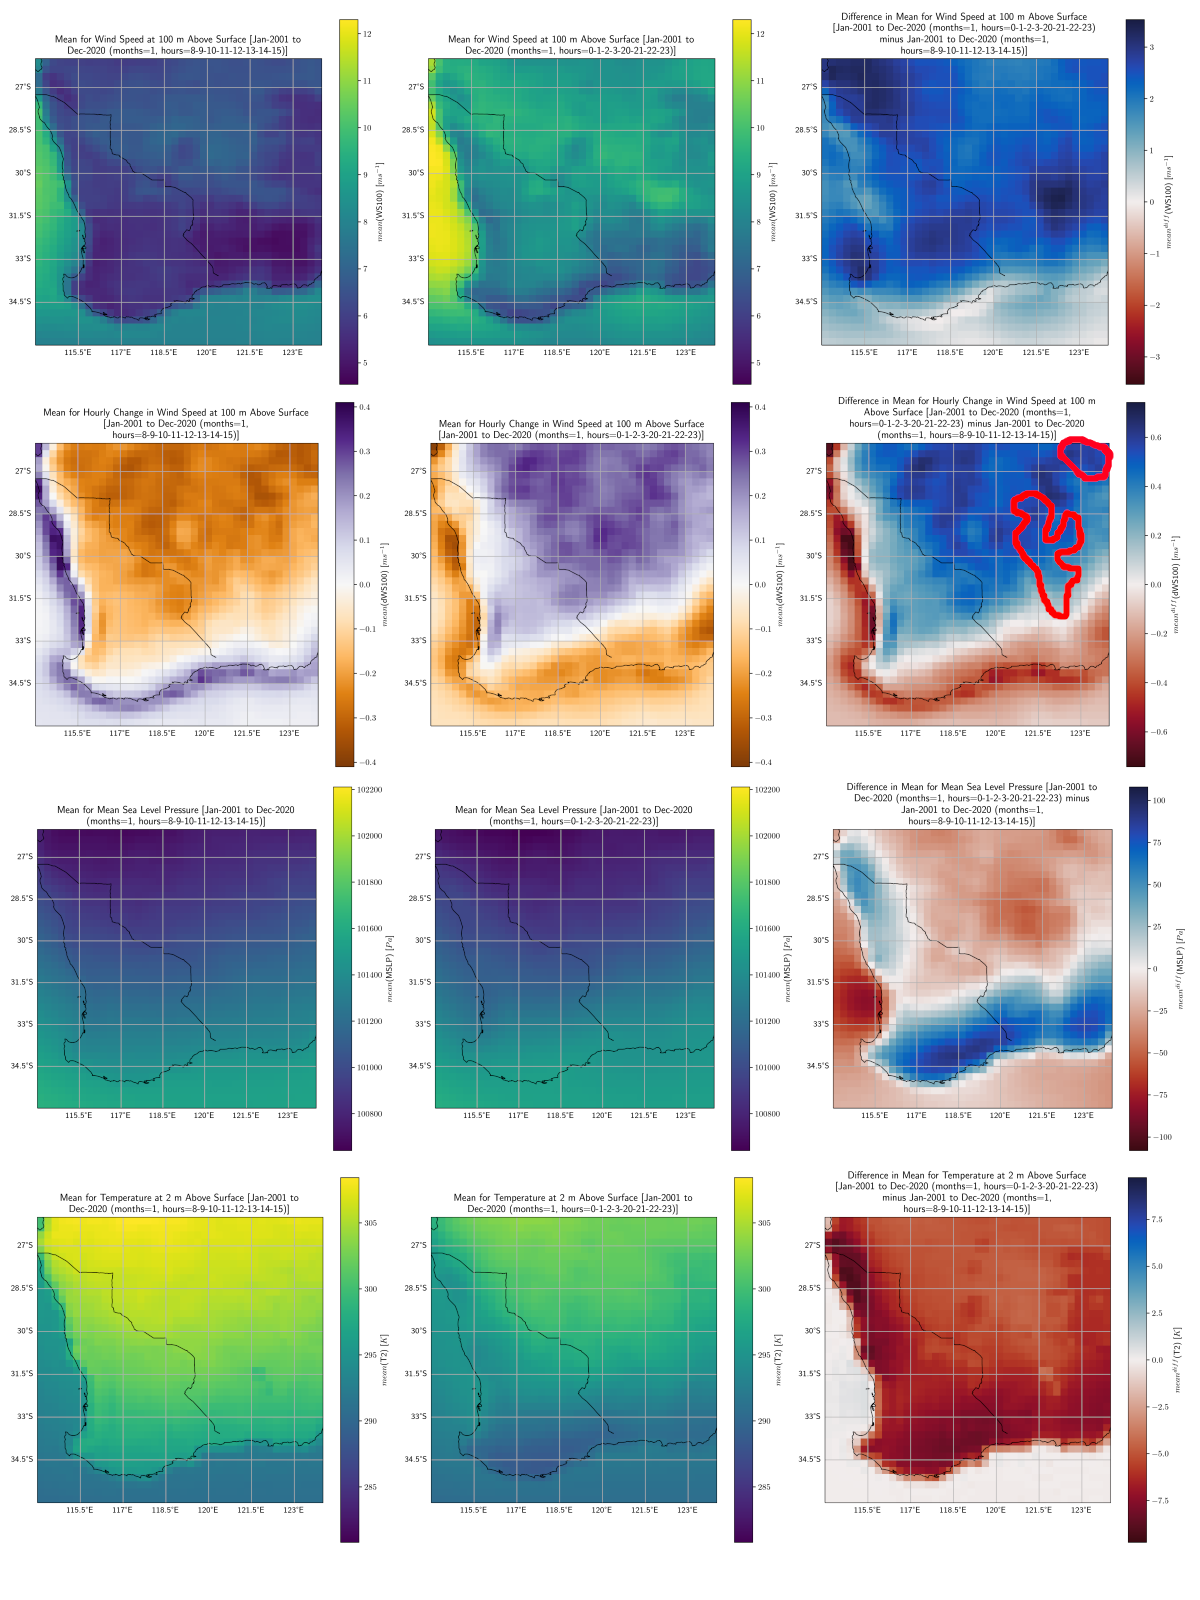
\includegraphics[width=0.9\textwidth]{wa_jan_comb_2.png}
	\caption[WA January means for selected variables 2]{January mean daytime and nighttime values for \acs{WS100}, \acs{dWS100}, \acs{MSLP} and \acs{T2}. Red markings indicate selected areas for \acs{dWS100} which are distinct from background trends but which deviate from orographic spatial patterns.}
	\label{fig:wa_jan_comb_2}
\end{figure}

\subsubsection{Localised anomalies.}

However, there are local-scale features which act contrary to this background trend. These are highlighted with red markings in Figure~\ref{fig:wa_jan_comb_1}.\footnote{The use of coloured markings with a thick outline somewhat distorts perception of these features. For an unmarked version of the figure, see Appendix~\ref{sec:unmarked}.} In these areas, \ac{VIEC} becomes increasingly negative (air movements are increasingly upwards directed) from daytime to nighttime despite the decrease in temperature, and there did not appear to be any localised anomalies in \ac{T2} which could explain this (see Figure~\ref{fig:wa_jan_comb_2}).

Interestingly, these \ac{VIEC}$^{diff}$ anomalies correspond to localised areas of positive \ac{NAC}$^{diff}$ (see Figure~\ref{fig:wa_jan_comb_1}). Given the suspected role of \ac{CIAD}, we turn to the question of whether this correlation primarily reflects a chance convergence of winds manifesting stronger upwards air movements which was then conducive towards cloud formation, or whether the actual condensation itself was responsible for the strengthening vertical motions.

\subsubsection{Contribution from lake evaporation.}

At least a few of these anomalies can be attributed to evaporation from ephemeral lakes\footnote{Although ephemeral, use of Google Earth satellite images confirms that these lakes contained water for all December months within the study period (and the water is presumably still there by January).}, which calls into question how relevant chance wind convergence would be on top of this. The lakes display a relatively low magnitude of evaporation decrease going from daytime to nighttime temperatures. This can be seen in the difference plot (right column) for \ac{NSE} in Figure~\ref{fig:wa_jan_comb_1} but for visual clarity, these lakes were marked in red for the nighttime plot (middle column) instead.

Furthermore, given the low magnitude of \ac{NSE} over these lakes relative to background trends, we would have expected increased water vapour \textit{divergence} via diffusion (positive \acs{VIDMF}$^{diff}$). But instead, what we observe is that these lakes correspond to areas of \textit{negative} \ac{VIDMF}$^{diff}$ (indicating increased water vapour \textit{convergence}). Given it is unlikely for a chance convergence of winds to coincidentally conform to the extents of the lakes, this flags the possibility of \ac{CIAD} as to our knowledge there has been no other proposed mechanism which would explain this anomaly. That is, continued evaporation combined with cooler temperatures during night time leads to increased atmospheric condensation, and under this may form a localised area of low pressure which advects air and moisture towards itself for sustenance.

\subsubsection{Implications for surface wind resource.} In studying implications for wind energy generation, we turn towards the \textit{hourly change} in 100 m wind speed (\acs{dWS100}). This allows us to analyse effects upon \acs{WS100} which may be slight and difficult to visually identify from a plot of \ac{WS100} itself since the signal is dominated by synoptic effects.

The spatial pattern observed for \acs{dWS100} corresponds mostly to the \ac{LSE} displayed in Figure~\ref{fig:orog}. Higher elevations are correlated with more negative d\ac{WS100} values during the daytime, more positive values during nighttime, and hence a greater magnitude of increase from day to night. Selected areas which display the opposite trends are highlighted with red markings in Figure~\ref{fig:wa_jan_comb_2}.\footnote{For an undistorted view, see the figure without markings in Appendix~\ref{sec:unmarked}.}

Interestingly, these areas correspond with the lakes identified earlier, and actually show an especially positive value for \acs{dWS100}$^{diff}$ (strengthening of winds). A more negative \ac{VIEC}$^{diff}$ (less conversion of internal and gravitational potential energy to kinetic) in these areas should imply a more negative \acs{dWS100}$^{diff}$ (weakening of winds) all other things equal, so it is not clear what is causing this anomaly. One possibility is that convection associated with increased \ac{NAC} (cloud formation) in these areas lead to favourable energy exchanges between the boundary layer and free atmosphere.

\subsection{Seasonal comparison for 1400 local time}

\ac{VIEC} mean values computed over 1400 \ac{LT} display a remarkable spatial correlation with that of \ac{NAC}. This is especially apparent near the coast for \ac{JJA} means, and in general for the difference plots between \ac{JJA} and \ac{DJF} (leftmost and rightmost columns in Figure~\ref{fig:wa_14_comb_1} respectively). More positive \ac{NAC} and \ac{NAC}$^{diff}$ values are correlated with more negative \ac{VIEC} and \ac{VIEC} $^{diff}$ values respectively. \ac{T2}$^{diff}$ (see Figure~\ref{fig:wa_14_comb_2}) shows a relatively uniform pattern and is consistent with the large-scale trend in \ac{VIEC} $^{diff}$ (warmer air tends to rise more), but it does not capture any of the smaller-scale trends that \ac{NAC}$^{diff}$ does.

\begin{figure}[!ht]
	\centering
	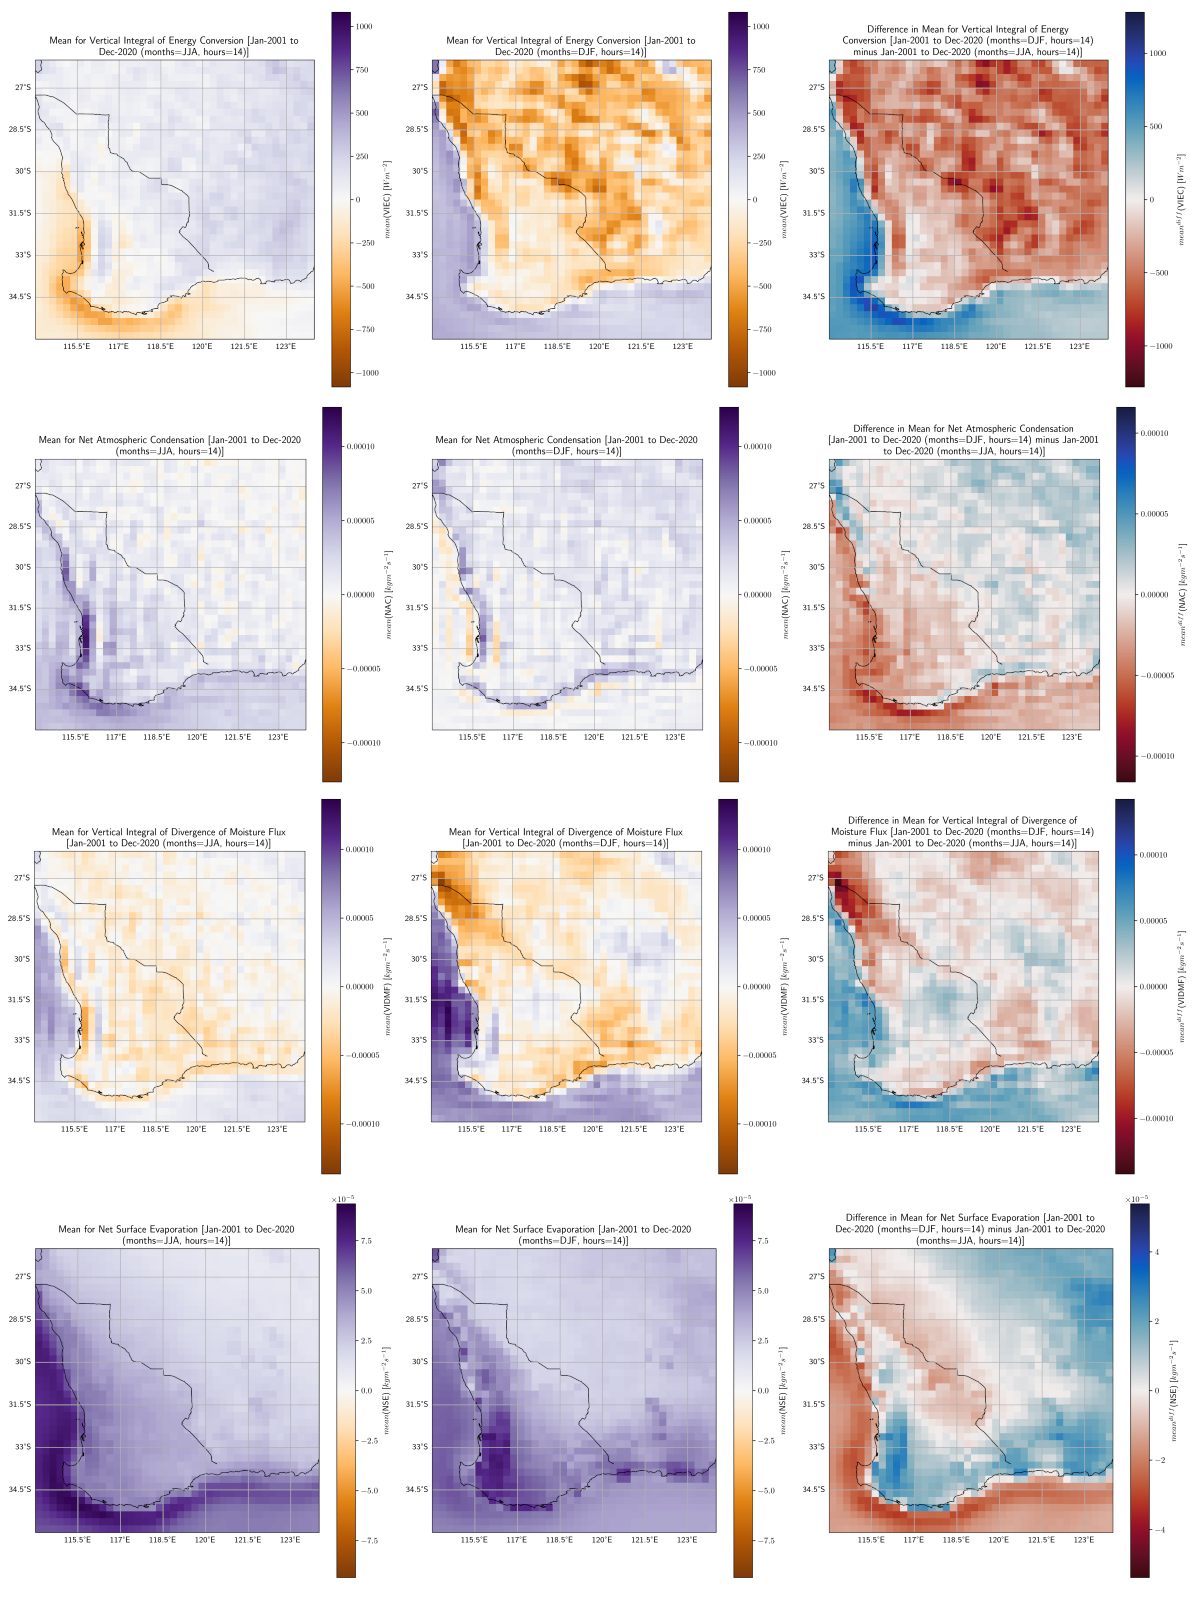
\includegraphics[width=0.9\textwidth]{wa_14_comb_1.png}
	\caption[WA 1400 means for selected variables 1]{1400 mean \acs{JJA} and \acs{DJF} values for \acs{VIEC}, \acs{NAC}, \acs{VIDMF} and \acs{NSE}.}
	\label{fig:wa_14_comb_1}
\end{figure}

\begin{figure}[!ht]
	\centering
	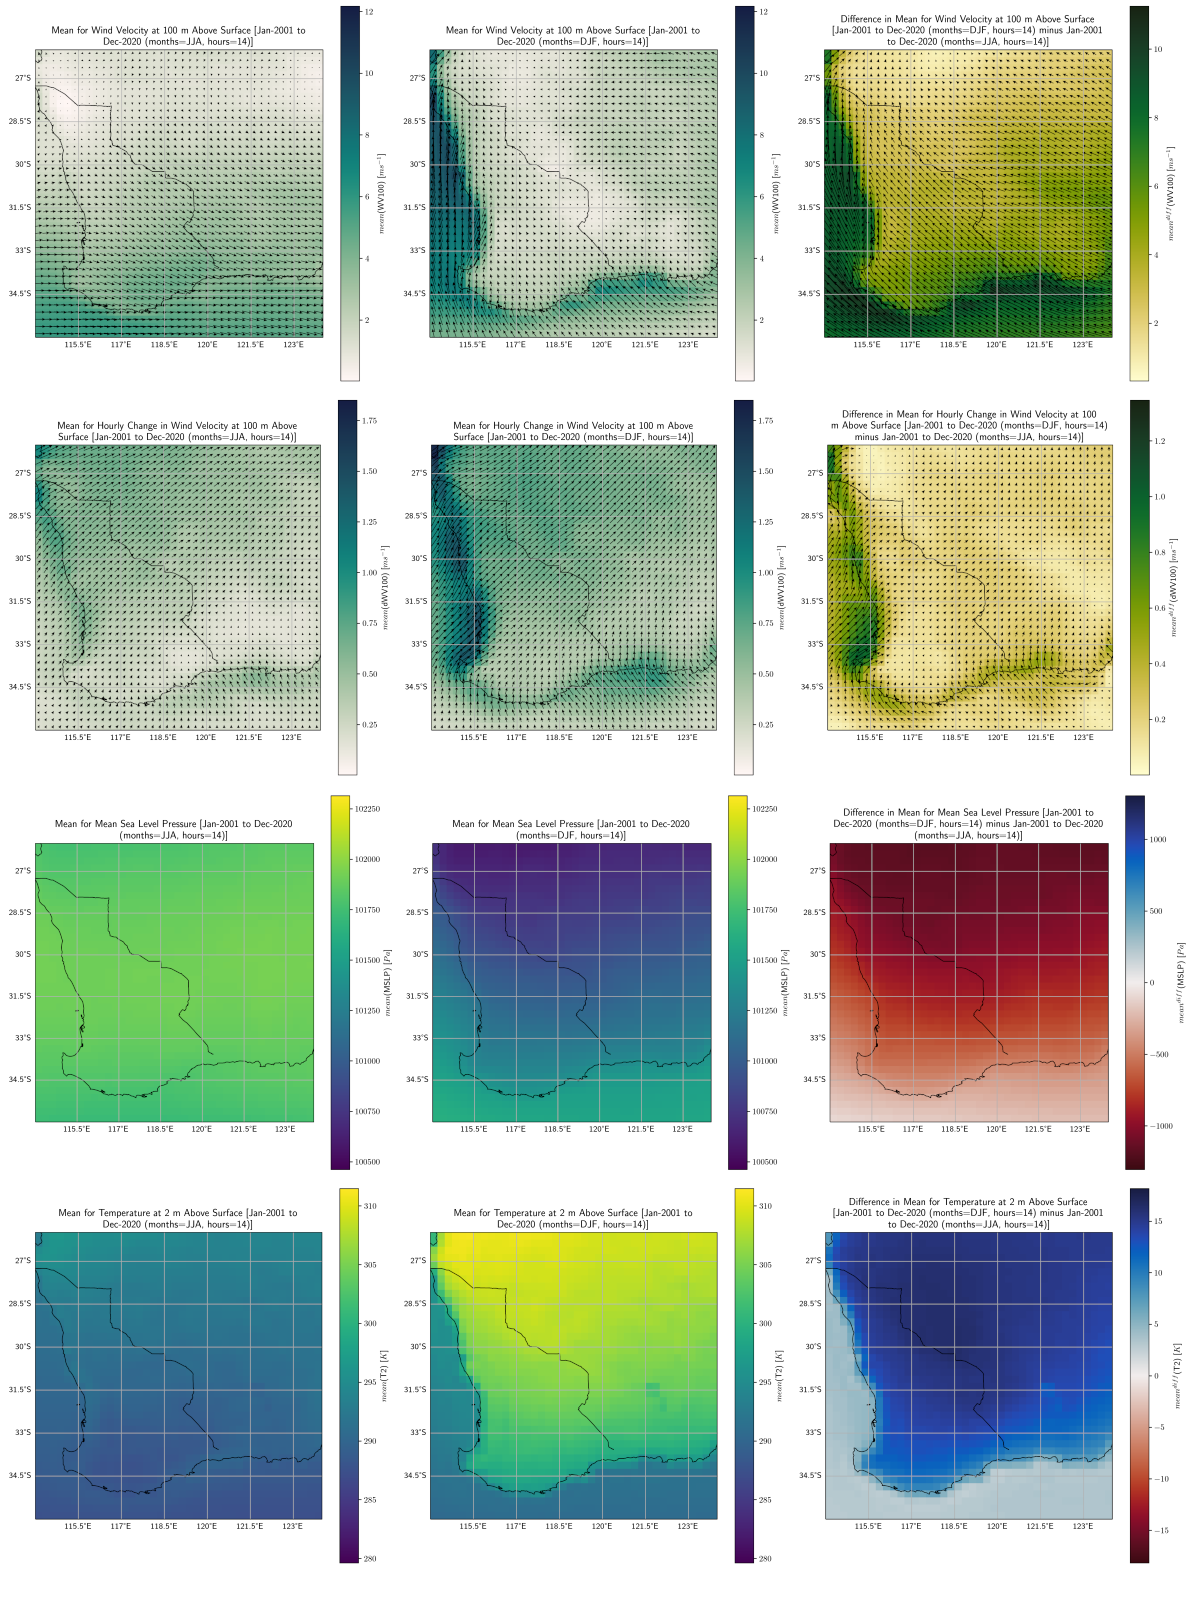
\includegraphics[width=0.9\textwidth]{wa_14_comb_2.png}
	\caption[WA 1400 means for selected variables 2]{1400 mean \acs{JJA} and \acs{DJF} values for \acs{WV100}, \acs{dWV100}, \acs{VIDMF} and \acs{NSE}.}
	\label{fig:wa_14_comb_2}
\end{figure}

We choose to display results for 1400 \ac{LT} here because results for this hour are most distinct, but the following is actually observed for all hours of the day in the hourly means analysis and all months of the year in the monthly means analysis (not shown):
\begin{itemize}
	\item For both \ac{JJA} and \ac{DJF} results, we observe that on the native side of the fence, most areas of negative \ac{VIDMF}$^{diff}$ (increased moisture \textit{convergence}) correlate with areas of positive \ac{NSE}$^{diff}$ (increased evaporation) but positive \ac{NAC}, contrary to what is expected from diffusion but consistent with \ac{CIAD}.
	\item None of the variables from which \ac{NAC} is derived display similar spatial patterns to \ac{VIEC} on large-scale (\ac{VIDMF} and \ac{NSE} for 1400 are displayed in Figure~\ref{fig:wa_14_comb_1}, \ac{TCWV} not shown at all). Only \ac{NAC} itself is similar to \ac{VIEC}.
	\item The concentrated band of negative \ac{VIEC} and positive \ac{NAC} means along the southwestern coastline for \ac{JJA} is present regardless of whether the band is upwind or downwind of the coastline, and whether the temperature gradients are producing a land or sea breeze (see \ac{T2} and \ac{dWV100} in Figure~\ref{fig:wa_14_comb_2} for 1400 \ac{LT} results).
\end{itemize}

The final point indicates that coastal orography and differential heating are unlikely to be responsible for the concentrated band along the southwestern coastline. And these points together conspire to heavily implicate the possibility of \ac{CIAD}.

One way in which negative \ac{VIEC} (rising air) could theoretically be concentrated along the coastline is if low-lying oceanic winds experience a sudden change in surface elevation and are deflected upwards from coastal cliffs and urban structures. But this does not explain why the observed bands in Figure~\ref{fig:wa_14_comb_1} extends out into the oceans, nor why the band is observed on the southernmost part of this region (around 35$^\circ$S) where winds are blowing from relatively high terrestrial ground to relatively low ocean surface (see \ac{WV100} in Figure~\ref{fig:wa_14_comb_2}). Furthermore, much stronger winds are blowing onshore during the \ac{DJF} months yet this coastal band is not observed for these months (compare \ac{VIEC} in Figure~\ref{fig:wa_14_comb_1} with \ac{WV100} in Figure~\ref{fig:wa_14_comb_2}). So it seems extremely unlikely that coastal orography is the cause.

Another way in which negative \ac{VIEC} (rising air) could theoretically be concentrated along the coastline is if a localised pressure gradient (arising from a temperature gradient) along the coastline adverse to the wind direction caused a bunching up of mass flux such that air had to be directed upwards. But results indicate the presence of this band regardless of the strength and direction of the coastline temperature gradient relative to prevailing winds. For the case of 1400 \ac{LT}, Figure~\ref{fig:wa_14_comb_2} displays a negligible coastal temperature gradient and magnitude of \ac{dWV100} in \ac{JJA}, yet the band exists for these months but not \ac{DJF} where these parameters are much more significant. So it also seems highly unlikely that differential heating is the cause.

\begin{figure}[!ht]
	\centering
	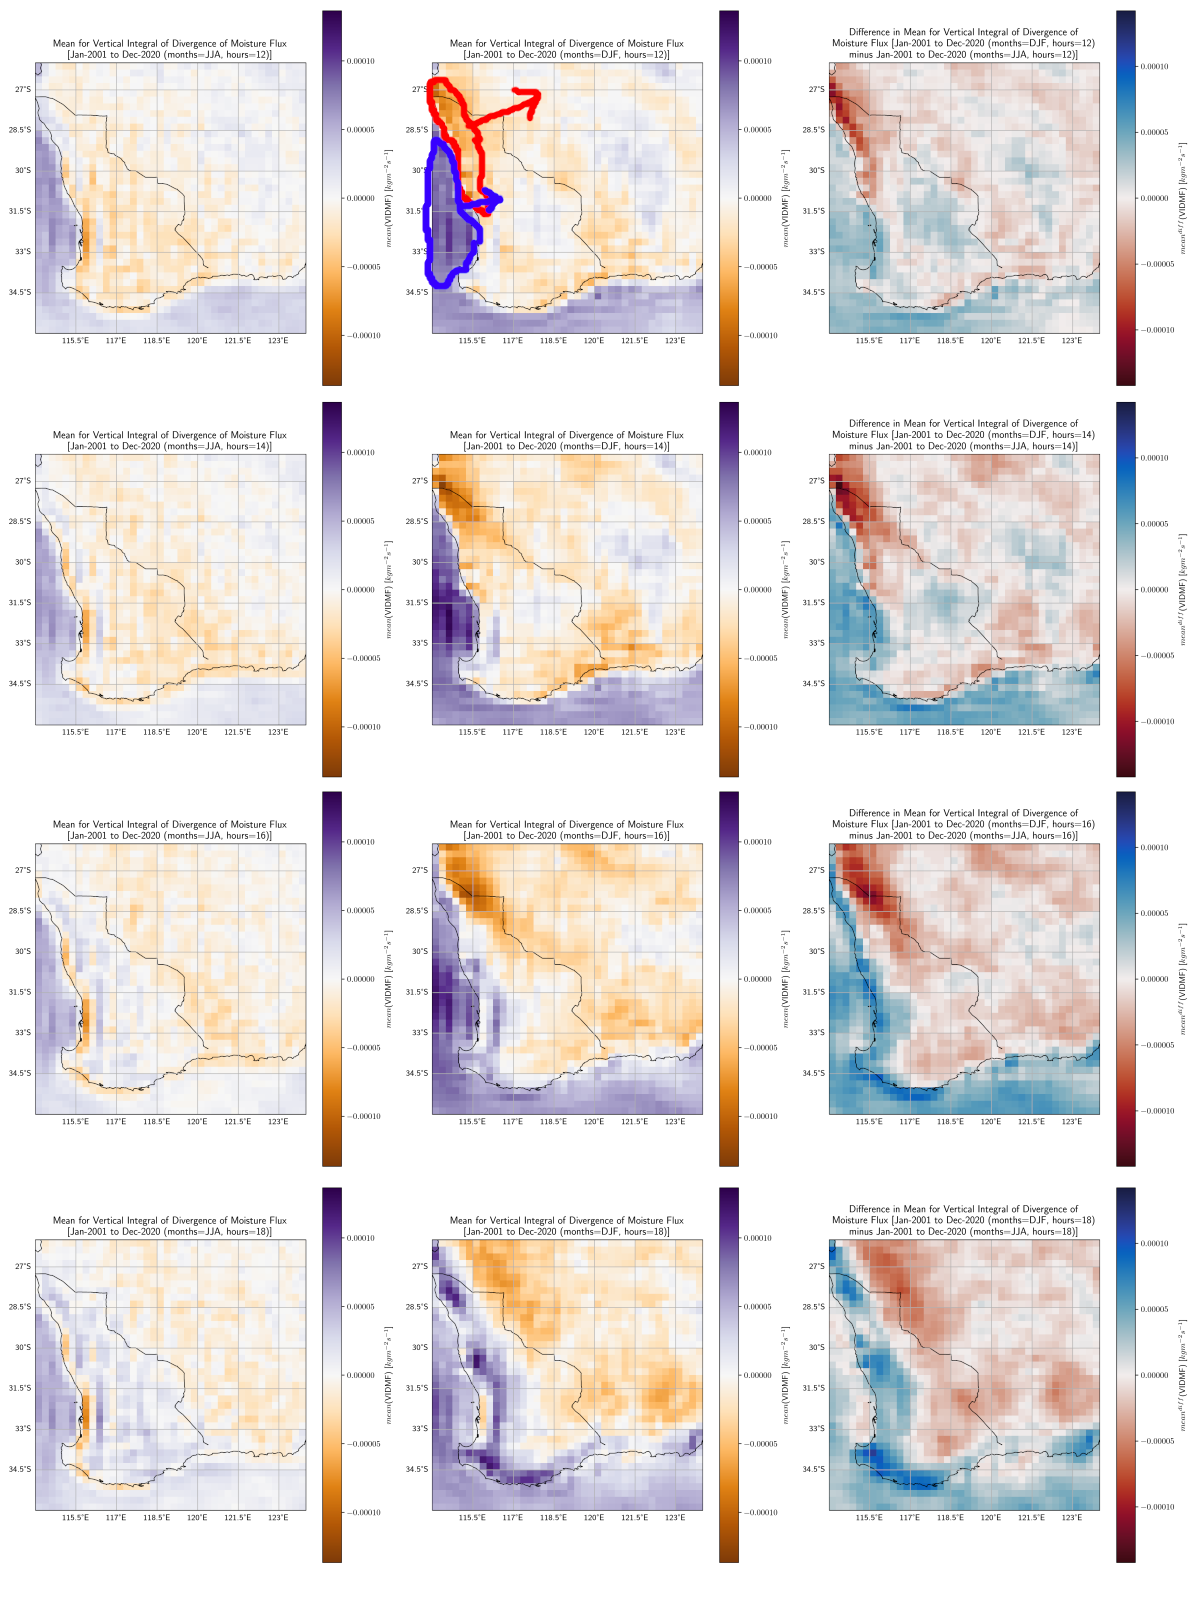
\includegraphics[width=0.9\textwidth]{wa_vidmf.png}
	\caption[WA 1400-1800 means for VIDMF]{1400-1800 mean \acs{JJA} and \acs{DJF} values for \acs{VIDMF}. Red and blue markings illustrate how moisture convergence and divergence respectively is initially concentrated near the coastline then moves inland as the day progresses, eventually reaching the point where convergence is concentrated on the native side of the fence.}
	\label{fig:wa_vidmf}
\end{figure}

One remaining explanation is that coastal condensation (positive \ac{NAC}) is \textit{driving} the band of upwards air movement (negative \ac{VIEC}) rather than the other way around (as per \ac{CIAD} theory), and that temperature gradients play a role in determining how much coastal moisture is available for condensation.

In this picture, the weaker winds from temperature gradients in \ac{JJA} compared to \ac{DJF} means the buildup of oceanic moisture along the coasts has a high condensation rate relative to moisture flux transport to inland areas. For the 1400 \ac{LT} case, this is reflected by low \ac{WV100} magnitude, low \ac{dWV100} magnitude and weak coastal \ac{T2} contrast in Figure~\ref{fig:wa_14_comb_2}, as well as a less positive \ac{VIDMF} offshore (ocean west of the coastline) despite higher \ac{NSE} in Figure~\ref{fig:wa_14_comb_1}. The result is that \ac{VIEC} displays a similar band to \ac{NAC} along the coast. This is also supported by the fact that the negative \ac{VIEC} band is absent from around 29$^\circ$S to 27$^\circ$S, which coincides with where \ac{dWV100} is especially strong.

On the other hand, stronger winds from temperature gradients in \ac{DJF} imply the converse. The ratio of inland moisture flux transport to coastal condensation rate is relatively high, so no coastal band of negative \ac{VIEC} is observed. Instead, there is increased condensation (relative to \ac{JJA}) on the native side of the fence, possibly due to higher \ac{SSHF}, and this is where negative \ac{VIEC} concentrates instead. This would seem to be supported by \ac{VIDMF} results which show for \ac{DJF} how moisture convergence (negative \ac{VIDMF}) moves inland ahead of moisture divergence (positive \ac{VIDMF}) as the day progresses, eventually reaching the point where convergence is concentrated on the native side of the fence (see Figure \ref{fig:wa_vidmf}).

\section{Central America}

\subsection{Seasonal comparison}

\subsubsection{Selected findings}

\subsection{Similar comparison}

\subsubsection{Study periods}
\label{sssec:period_seas_ca}

For \ac{CA}, the selected periods for the similar comparison was from Jan-2002 to Dec-2006 and from Jan-2014 to Dec-2018.

The pair of Jan-2002 to Dec-2006 and Jan-2014 to Dec-2018 was deemed most appropriate since these periods had comparable averages in relevant climate indices and appear to span across the same phase of the relevant atmospheric oscillations. This was true for all of the relevant indices: \ac{AMOI}, \ac{PDOI}, \ac{ONI} (for \ac{ENSO}), and the \ac{EPOI}. The \ac{AOI} and \ac{NAOI} over these periods (not shown) also appeared to span across the same phase but had 5-year averages with slightly higher disparities (but these disparities were nevertheless small in terms of the characteristic size of the oscillations). The \ac{DMI} and the \ac{AAOI} (not shown) over these periods, on the other hand, were considerably different, but these were assumed not to be a major factor due to the distance of the Indian Ocean and Antarctica from the Americas\footnote{Significant effects due to teleconnections are theoretically possible but we have assumed this isn't the case here}.

The similarity between these periods is particularly remarkable because even the monthly values and 5-year averages for the \ac{ONI} (which has irregular oscillations) display a similar time evolution pattern. Both periods begin with the conclusion of an El Nino event and end past halfway into an La Nina event, and fully covers another La Nina event in between. The period from Jan-2014 to Dec-2018 contains an additional El Nino event not found in the period from Jan-2002 to Dec-2006 but this appears to mostly be a technicality with the definition of an El Nino event. A look at the monthly values reveals a spike in the \ac{ONI} which could have qualified as an El Nino event under slightly relaxed definitions. Furthermore, the monthly values between the starting El Nino event and ending La Nina event are almost mirror images of each other.

In the case of Costa Rica, although remote sensing indicates that the rate of forest cover increase here was highest during the 1990s, leaf area index data derived from the \ac{AVHRR} instrument (not shown) for this region showed considerable noise and disagreement with \ac{MODIS} (the more advanced instrument). Given these factors, this set of study periods was also desirable because it was completely contained within the \ac{MODIS} coverage period. In addition to this, a land cover classification study by \citet{marx2017} using Landsat and \ac{UAV} data in lowland Costa Rica suggested an 11-year period for a pasture to transition into secondary forest, so a 13 year difference between selected periods corresponds well with our goals for studying the effects of \ac{LCC}.

\subsubsection{Selected findings}

\section{Northern Brazil}

\subsection{Seasonal comparison}

\subsubsection{Selected findings}

\subsection{Similar comparison}

\subsubsection{Study periods}

For \ac{NB}, the selected periods for the similar comparison was from Jan-2002 to Dec-2006 and from Jan-2014 to Dec-2018 (for the same reasons highlighted in Section~\ref{sssec:period_seas_ca} for \ac{CA}.

\subsubsection{Selected findings}









Should include a reiteration of the experiments, and their outcome.  Together with a description (discussion).  Preamble should include a reminder of the aims and objectives together with a list of experiments to achieve these.  Should include many charts and other visualization with appropriate descriptions.  

\Blindtext

\section*{Summary}
\blindtext\enlargethispage{\baselineskip} % so you do not get a single line in another pag